\documentclass[9pt]{beamer}

\mode<presentation> {

% The Beamer class comes with a number of default slide themes
% which change the colors and layouts of slides. Below this is a list
% of all the themes, uncomment each in turn to see what they look like.

%\usetheme{default}
%\usetheme{AnnArbor}
%\usetheme{Antibes}
%\usetheme{Bergen}
%\usetheme{Berkeley}
\usetheme{Berlin}
%\usetheme{Boadilla}
%\usetheme{CambridgeUS}
%\usetheme{Copenhagen}
%\usetheme{Darmstadt}
%\usetheme{Dresden}
%\usetheme{Frankfurt}
%\usetheme{Goettingen}
%\usetheme{Hannover}
%\usetheme{Ilmenau}
%\usetheme{JuanLesPins}
%\usetheme{Luebeck}
%\usetheme{Madrid}
%\usetheme{Malmoe}
%\usetheme{Marburg}
%\usetheme{Montpellier}
%\usetheme{PaloAlto}
%\usetheme{Pittsburgh}
%\usetheme{Rochester}
%\usetheme{Singapore}
%\usetheme{Szeged}
%\usetheme{Warsaw}

% As well as themes, the Beamer class has a number of color themes
% for any slide theme. Uncomment each of these in turn to see how it
% changes the colors of your current slide theme.

%\usecolortheme{albatross}
%\usecolortheme{beaver}
%\usecolortheme{beetle}
%\usecolortheme{crane}
%\usecolortheme{dolphin}
\usecolortheme{dove}
%\usecolortheme{fly}
%\usecolortheme{lily}
%\usecolortheme{orchid}
%\usecolortheme{rose}
%\usecolortheme{seagull}
%\usecolortheme{seahorse}
%\usecolortheme{whale}
%\usecolortheme{wolverine}

%\setbeamertemplate{footline} % To remove the footer line in all slides uncomment this line
%\setbeamertemplate{footline}[page number] % To replace the footer line in all slides with a simple slide count uncomment this line

%\setbeamertemplate{navigation symbols}{} % To remove the navigation symbols from the bottom of all slides uncomment this line
}

\usepackage{units}
\usepackage{extpfeil}
\usepackage{extarrows} %Allows long equation signs
\usepackage{graphicx} % Allows including images
\usepackage{booktabs} % Allows the use of \toprule, \midrule and \bottomrule in tables
\usepackage{physics}
\usepackage{tikz}
\usepackage{cite}
%花体字母
\usepackage{amsthm,amsmath,amssymb}
\usepackage{mathrsfs}
\usepackage{dutchcal}
\usepackage{circuitikz}
\usepackage{eqnarray}
\usepackage{multirow}
%----------------------------------------------------------------------------------------
%	TITLE PAGE
%----------------------------------------------------------------------------------------

\title[VP260 RC]{VP260 Recitation Class 7} % The short title appears at the bottom of every slide, the full title is only on the title page

\author{Shijie Zhong} % Your name
\institute[UM-SJTU JI] % Your institution as it will appear on the bottom of every slide, may be shorthand to save space
{
    University of Michigan - Shanghai Jiao Tong University Joint Institute\\% Your institution for the title page
\medskip
}
\date{\today} % Date, can be changed to a custom date

\begin{document}

\begin{frame}
    \titlepage % Print the title page as the first slide
\end{frame}


%----------------------------------------------------------------------------------------
%	 SECTION 1
%----------------------------------------------------------------------------------------

\section{Fundamental Concepts} % Section title slide, unnumbered

\begin{frame}{The Helmholtz's Theorem}
    \begin{beamerboxesrounded}[shadow=true]{\bf The Helmholtz's Theorem (not rigorous)}
        Let $\va{F}(\va{r})$  be a continuous vector field, which is continuously partial differentiable, then $\va{F}(\va{r})$ can be uniquely decomposed into two components,
        \begin{equation}
            \va{F} (\va{r}) = -\grad{\varphi(\va{r})} + \curl{\va{A}(\va{r})}.
        \end{equation}
    \end{beamerboxesrounded}

    \begin{itemize}
        \item The first component $\varphi(\va{r})$ is called scalar potential and the second component $\va{A} (\va{r})$ is called vector potential.
        \item Why?
        \begin{equation}
            \div{\va{F}} = \div(-\grad{\varphi} + \curl{\va{A}}) = -\laplacian{\varphi}
        \end{equation}
        \begin{equation}
            \curl{\va{F}} = \curl(-\grad{\varphi} + \curl{\va{A}}) = \curl(\curl{\va{A}})
        \end{equation}
    \end{itemize}

\end{frame}

\begin{frame}{Scalar and Vector Potentials}
    \begin{beamerboxesrounded}[shadow=true]{\bf Maxwell's Equations}
        \begin{table}[htbp]
            \centering
            \begin{tabular}{ll}
            \addlinespace[1em]
            $\div{\va{E}} = \frac{\rho}{\epsilon_0}$ & $\curl{\va{E}}=-\pdv{\va{B}}{t}$ \\ \addlinespace[1em]
             $\div{\va{B}} = 0$ & $\curl{\va{B}}=\mu_0 \va{J}+ \mu_0 \epsilon_0 \pdv{\va{E}}{t}$ 
            \end{tabular}
        \end{table}
    \end{beamerboxesrounded}
    \vspace{.5em}
    \begin{beamerboxesrounded}[shadow=true]{\bf Vector Potential}
        \begin{equation}
            \va{B} = \curl \va{A}
        \end{equation}
        \begin{equation}
            \va{E} = -\grad V - \pdv{\va{A}}{t}
        \end{equation}
    \end{beamerboxesrounded}
\end{frame}

\begin{frame}{Scalar and Vector Potential}
    \begin{beamerboxesrounded}[shadow=true]{\bf Maxwell's Equations}
        \begin{equation}
            \nabla^{2} V+\frac{\partial}{\partial t}(\mathbf{\nabla} \cdot \mathbf{A})=-\frac{1}{\epsilon_{0}} \rho
        \end{equation}
        \begin{equation}
            \left(\nabla^{2} \mathbf{A}-\mu_{0} \epsilon_{0} \frac{\partial^{2} \mathbf{A}}{\partial t^{2}}\right)-\nabla\left(\mathbf{\nabla} \cdot \mathbf{A}+\mu_{0} \epsilon_{0} \frac{\partial V}{\partial t}\right)=-\mu_{0} \mathbf{J}
        \end{equation}
    \end{beamerboxesrounded}    
    \vspace{.5em}
    \begin{beamerboxesrounded}[shadow=true]{\bf Gauge Transform}
        \begin{equation}
            \mathbf{A}'=\mathbf{A}+\nabla \lambda
        \end{equation}     
        \begin{equation}
            V'=V-\frac{\partial \lambda}{\partial t}
        \end{equation}   

        Help to adjust $\div\va{A}$.
        \begin{itemize}
            \item Magnetostatics: choose $\div\va{A}=0$
        \end{itemize}
    \end{beamerboxesrounded}
\end{frame}

\begin{frame}{Gauge Transform}
    \begin{beamerboxesrounded}[shadow=true]{\bf Lorenz Gauge}
        To eliminate the middle term in Eq(4):
        \begin{equation*}
            \div \va{A} = -\mu_0\epsilon_0\pdv{V}{t}
        \end{equation*}
        Eq(3,4) becomes (symmetric):
        \begin{align*}
            \nabla^{2} \mathbf{A}-\mu_{0} \epsilon_{0} \frac{\partial^{2} \mathbf{A}}{\partial t^{2}} &= -\mu_{0} \mathbf{J} \\ 
            \nabla^{2} V-\mu_{0} \epsilon_{0} \frac{\partial^{2} V}{\partial t^{2}} &= -\frac{1}{\epsilon_{0}} \rho
        \end{align*}
    \end{beamerboxesrounded}
\end{frame}


\begin{frame}{Gauge Transform}
    \begin{beamerboxesrounded}[shadow=true]{\bf Coulomb Gauge (Magnetostatics)}
        \begin{equation*}
            \div\va{A} = 0
        \end{equation*}
        Eq(3) becomes (Poisson's equation):
        \begin{equation*}
            \nabla^{2} V=-\frac{1}{\epsilon_{0}} \rho
        \end{equation*}
        Eq(4) becomes:
        \begin{equation*}
            \nabla^{2} \mathbf{A}-\mu_{0} \epsilon_{0} \frac{\partial^{2} \mathbf{A}}{\partial t^{2}}=-\mu_{0} \mathbf{J}+\mu_{0} \epsilon_{0} \nabla\left(\frac{\partial V}{\partial t}\right)
        \end{equation*}

        \begin{itemize}
            \item Easy to calculate scalar potential ($V$)
            \item Hard to calculate vector potential ($\va{A}$)
        \end{itemize}
    \end{beamerboxesrounded}
\end{frame}
%There is a very peculiar thing about the scalar potential in the Coulomb gauge: it is determined by the distribution of charge right now. If I move an electron in my laboratory, the potential V on the moon immediately records this change. That sounds particularly odd in the light of special relativity, which allows no message to travel faster than c. The point is that V by itself is not a physically measurable quantity—all the man in the moon can measure is E, and that involves A as well (Eq. 10.3). Somehow it is built into the vector potential (in the Coulomb gauge) that whereas V instantaneously reflects all changes in ρ, the combination −∇V − (∂A/∂t) does not; E will change only after sufficient time has elapsed for the “news” to arrive.1

\begin{frame}{Gauge Transform}
    Recall that $\curl \va{B} = \mu_0 \va{J}$, then we can get 
    \begin{equation*}
        \nabla \times \mathbf{B}=\nabla \times(\nabla \times \mid \mathbf{A})=\nabla(\nabla \cdot \mathbf{A})-\nabla^{2} \mathbf{A} = -\nabla^2 \va{A} = \mu_{0} \mathbf{J}
    \end{equation*}

    Similar to Poisson's equation ($-\nabla^2 V = \rho/\epsilon_0$), then the solution should be:
    \begin{equation*}
        \mathbf{A}(\mathbf{r})=\frac{\mu_{0}}{4 \pi} \int \frac{\mathbf{J}\left(\mathbf{r}^{\prime}\right)}{r} \dd \tau^{\prime}
    \end{equation*}
    For line current,
    \begin{equation*}
        \mathbf{A}=\frac{\mu_{0} I}{4 \pi} \oint \frac{\dd \mathbf{l}}{r}
    \end{equation*}

    Useful to calculate the magnetic flux through $\va{B}$.
\end{frame}


\begin{frame}{Inductance (unit: H)}
    \begin{equation*}
        \Phi_{2}=\int \mathbf{B}_{1} \cdot \dd \mathbf{a}_{2}=\int\left(\mathbf{\nabla} \times \mathbf{A}_{1}\right) \cdot \dd \mathbf{a}_{2}=\oint \mathbf{A}_{1} \cdot \dd \mathbf{l}_{2} =\frac{\mu_{0} I_{1}}{4 \pi} \oint\left(\oint \frac{\dd \mathbf{l}_{1}}{r}\right) \cdot \dd \mathbf{l}_{2}
    \end{equation*}
    \begin{beamerboxesrounded}[shadow=true]{\bf Mutual Inductance}
        \begin{equation}
            M_{21}=\frac{\mu_{0}}{4 \pi} \oint \oint \frac{d \mathbf{l}_{1} \cdot d \mathbf{l}_{2}}{r}
        \end{equation}
        \begin{equation}
            M_{21} = M_{12} 
        \end{equation}

        \begin{itemize}
            \item Geometrical quantity
        \end{itemize}
    \end{beamerboxesrounded}

    \begin{beamerboxesrounded}[shadow=true]{\bf Self Inductance}
        \begin{equation}
            \Phi = L I
        \end{equation}
        \begin{equation}
            \varepsilon = - L \dv*{I}{t} 
        \end{equation}

        Pay attention to the direction (potential drop through inductor).
    \end{beamerboxesrounded}
\end{frame}

\begin{frame}{Energy}
    \begin{itemize}
        \item Inductor: $W_L = \frac{1}{2} L I^2$
        \item Magnetic field energy density: $u = \frac{B^2}{2 \mu}$, $\mu=\mu_r\mu_0$
        \item Electric field energy density: $u=\frac{1}{2}\epsilon_r\epsilon_0E^2$
    \end{itemize}
\end{frame}

\begin{frame}{RL, LC, RLC Circuits}
    \begin{table}[htbp]
        \centering
        \begin{tabular}{l c l}
            \toprule
            RC & $i(t)=\epsilon/R(1-exp(-t/\tau))$ & $\tau=RC$ \\ \addlinespace[1em]
            RL & $i(t)=\epsilon/R(1-exp(-t/\tau))$ & $\tau=L/R$ \\ \addlinespace[1em] 
            LC & $q(t) = A\sin(\omega_0 t) + B\cos(\omega_0 t)$ & $\omega_0 = 1\sqrt{LC}$\\ \addlinespace[1em]
            \multirow{3}{*}{RLC} & \multirow{3}{*}{$\frac{d^{2} I(t)}{d t^{2}}+\frac{R}{L} \frac{d I(t)}{d t}+\frac{1}{L C} I(t)=0$} & Underdamped \\ 
            &&Critical damping \\
            &&Overdamped \\
            \bottomrule
        \end{tabular}
    \end{table}
\end{frame}

\begin{frame}{AC Circuit}
    \begin{beamerboxesrounded}[shadow=true]{\bf AC Current}
        \begin{align}
            i(t) &= I\cos(\omega t + \phi) \\
            i(t) &= \mathit{Re}\{ I exp(j(\omega t + \phi))\} = \mathit{Re}\{ A exp(j\omega t)\}
        \end{align}
    \end{beamerboxesrounded}
    \vspace{.5em}
    \begin{itemize}
        \item Rectified average current: $I_{rav} = \frac{1}{T}\int_{t_1}^{t_1+T}\abs{i(t)}\dd t = \frac{2}{\pi}I$
        \item Root-mean-square current: $I_{rms} = \sqrt{\frac{1}{T}\int_{t_1}^{t_1+T}i^2(t)\dd t} = \frac{I}{\sqrt{2}}$
    \end{itemize}
\end{frame}

\begin{frame}{Elements in AC}
    \begin{table}[htbp]
        \centering
        \begin{tabular}{l c c}
            \toprule
            Elements & Impedance & Phase \\ 
            \midrule
            R & $R$ & 0 \\  
            L & $j\omega L $ & $\pi/2$ \\ 
            C & $1/(j \omega C)$ & $-\pi/2$ \\ 
            \bottomrule
        \end{tabular}
    \end{table}
    
    \begin{beamerboxesrounded}[shadow=true]{\bf Resonance}
        \begin{equation}
            \abs{Z} = \sqrt{R^2+(\omega L - \frac{1}{\omega C})^2 }
        \end{equation}
        Resonance happens when $\omega_0 = \frac{1}{LC}$        
    \end{beamerboxesrounded}

    \begin{beamerboxesrounded}[shadow=true]{\bf Power}
        \begin{equation}
            \overline{P} = \frac{1}{T} \int_{t}^{t+T}vi \dd t = V_{rms} I_{rms} 
        \end{equation}
    \end{beamerboxesrounded}
\end{frame}

%----------------------------------------------------------------------------------------
%	 Section 2
%----------------------------------------------------------------------------------------

\section{Exercise}

\begin{frame}{Exercise 1}
$B_{x}=-k x, B_{y}=0, B_{z}=B_{0}+k z$ ($k,B_0 > 0$). Rigid frame ABCD (mass $m$, width $a$, inductance $L$, without resistance) is released at $t=0$, please find out the following motion (neglect the motional emf of side AB and CD). 
\begin{figure}[htbp]
    \centering
    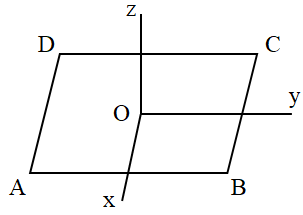
\includegraphics[scale=0.8]{images/ex1.png}
\end{figure}
\end{frame}

\begin{frame}{Exercise 2}
    Find the energy stored in a section of length $l$ of a long solenoid (radius $R,$ current $I, n$ turns per unit length)
    \begin{itemize}
        \item[(a)] using $W=\frac{1}{2}LI^2$ 
        \item[(b)] using $W=\frac{1}{2}\oint(\va{A}\cdot\va{I})\dd l$ 
        \item[(c)] using $W=\frac{1}{2\mu_0}\int_{all \ space}B^2\dd \tau$;
        \item[(d)] using $W=\frac{1}{2 \mu_{0}}\left[\int_{\mathcal{V}} B^{2} d \tau-\oint_{\mathcal{S}}(\mathbf{A} \times \mathbf{B}) \cdot d \mathbf{a}\right]$ (take as your volume the cylindrical tube from radius $a<R$ out to radius $b>R$ ).
    \end{itemize}
\end{frame}

\begin{frame}{Exercise 3}
    Solve the following circuit.

\begin{figure}[htbp]
    \centering
    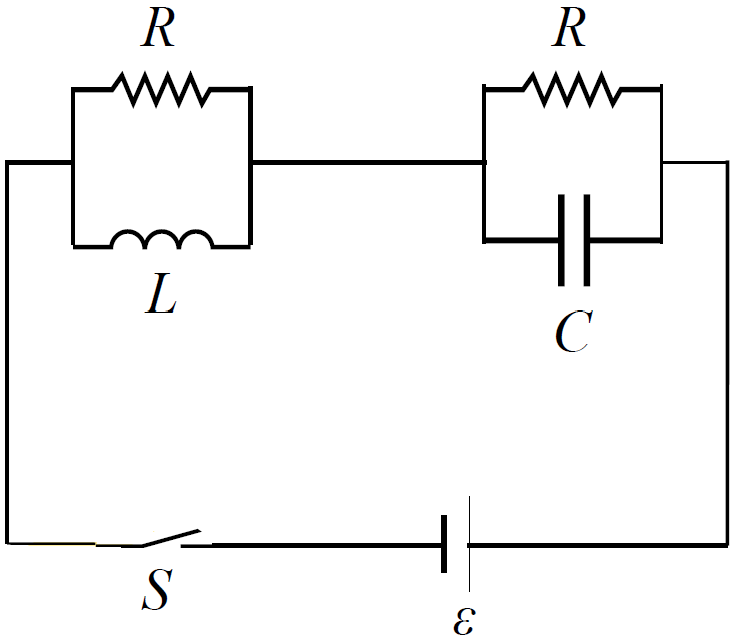
\includegraphics[scale=0.6]{images/ex3.png}
\end{figure}
\end{frame}


%----------------------------------------------------------------------------------------
%	 CLOSING/SUPPLEMENTARY SLIDES
%----------------------------------------------------------------------------------------
\section{Appendix}


\begin{frame}
    \begin{center}
        \LARGE\bf Thanks for listening!
    \end{center}
\end{frame}


%----------------------------------------------------------------------------------------

\begin{frame}{\bf References}
    \nocite{*} % Display all references regardless of if they were cited
    \bibliographystyle{plain}
    \bibliography{example.bib}
\end{frame}

\end{document}

